% \newcommand{\testsuccess}{\symbol{"2B45}}
% \newcommand{\testfail}{\symbol{"2718}}

\newcommand{\testsuccess}{\cmark{}}
\newcommand{\testfail}{\xmark{}}

% \pagebreak
% \newgeometry{margin=2cm}
% \begin{sidewaysfigure}
%     \centering
%     \makebox[\linewidth][c]{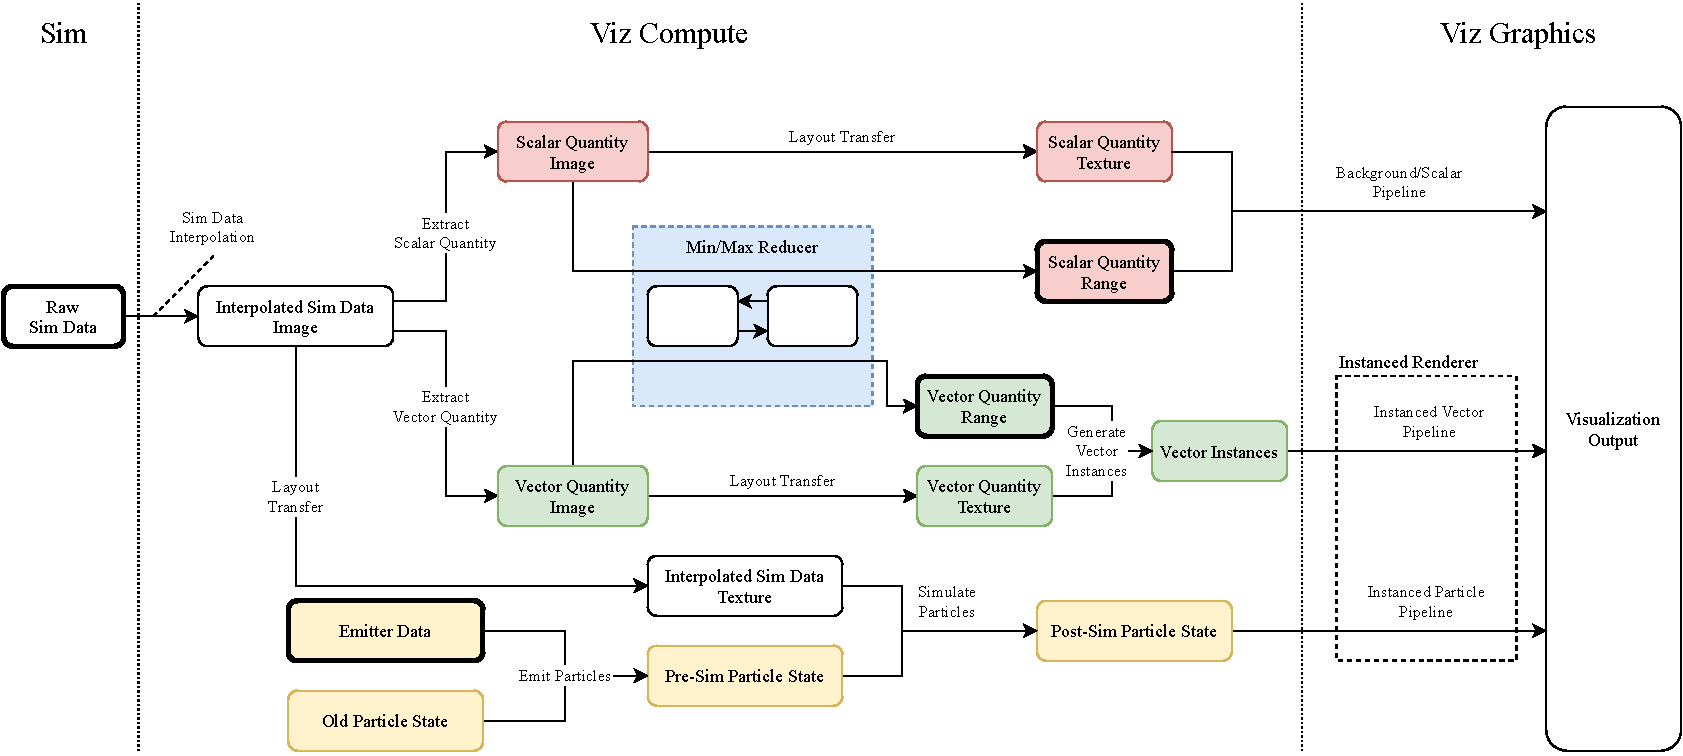
\includegraphics[width=\linewidth]{Ch48Implementation/figures/FinalReport_VizData.pdf}}
%     \caption{Data Transformation Diagram showing the data flow for the Visualization}
%     \label{fig:VizDataTransform}
% \end{sidewaysfigure}
% \restoregeometry
% \pagebreak

\begin{sidewaystable}
    \centering
    \begin{tabular}{ll|c|c|c}
        ID & Description & Expected & Output & Result \\
        \hline
        \newtest{}\label{test:unit:compare:identical} & \shell{compare}: identical states & No difference & No difference & \testsuccess{} \\
        \newtest{}\label{test:unit:compare:different} & \shell{compare}: Original input to original target output & Some difference & Some difference & \testsuccess{} \\
        \newtest{}\label{test:unit:renderppm} & \shell{renderppm}: render state vorticity & Equal to original program & Equal to original program & \testsuccess{} \\
        \newtest{}\label{test:unit:makeinput} & \shell{makeinput}: generate an input file from a PNG & Valid simulation state & Valid simulation state & \testsuccess{} \\
        \newtest{}\label{test:unit:fixedtime} & \shell{fixedtime}: simulate from an input state for 25 seconds. & Valid simulation state & Valid simulation state & \testsuccess{} \\
        \newtest{}\label{test:unit:run} & \shell{run}: visualize a simulation from an input state for 25 seconds. & Valid simulation state & Valid simulation state & \testsuccess{} \\
    \end{tabular}
    \caption{Unit Tests}
    \label{tab:unittests}
\end{sidewaystable}
